\chapterimage{chapter_head_2.pdf} % Chapter heading image

\chapter{Hidden Services}

\section{Rendezvous Points and hidden services}
Rendezvous points are a building block for location-hidden services (also known as responder anonymity) in the Tor net- work. Location-hidden services allow Bob to offer a TCP service, such as a webserver, without revealing his IP address.\cite{tor_paper}

We provide location-hiding for Bob by allowing him to advertise several onion routers (his introduction points) as contact points.\cite{tor_paper}
He may do this on any robust efficient key-value lookup system with authenticated updates, such as a distributed hash table (DHT) like CFS.\cite{tor_paper} \footnote{ This DHTs is distributed across many Tor relays (HSDirs) Any regular Tor relay may work as HSDir, anyone who deploys such HSDir nodes can also harvest onion addresses from it. The adversary may find addresses that have not been publicly shared ever. \cite{tor_slideshare}}
Alice, the client, chooses an OR as her rendezvous point. She connects to one of Bob’s introduction points, informs him of her rendezvous point, and then waits for him to connect to the rendezvous point.\cite{tor_paper}
\subsection{Rendezvous points in Tor}
The following steps are performed on behalf of Alice and Bob by their local OPs \cite{tor_paper} :
\begin{itemize}
	\item Bob generates a long-term public key\footnote{The hostname is just the (truncated) hash of the public key\cite{stackDNS}} pair to identify his service.
	\item Bob chooses some introduction points, and advertises them on the lookup service, signing the advertisement with his public key. He can add more later.
	\item Bob builds a circuit to each of his introduction points, and tells them to wait for requests.
	\item Alice learns about Bob’s service out of band (perhaps Bob told her, or she found it on a website). She retrieves the details of Bob’s service from the lookup service. If Alice wants to access Bob’s service anonymously, she must connect to the lookup service via Tor.
	\item Alice chooses an OR as the rendezvous point (RP) for her connection to Bob’s service. She builds a circuit to the RP, and gives it a randomly chosen “\underline{rendezvous cookie}” to recognize Bob.
	\item Alice opens an anonymous stream to one of Bob’s introduction points, and gives it a message (encrypted with Bob’s public key) telling it about herself, her RP and rendezvous cookie, and the start of a DH handshake. The introduction point sends the message to Bob.
	\item If Bob wants to talk to Alice, he builds a circuit to Al- ice’s RP and sends the rendezvous cookie, the second half of the DH handshake, and a hash of the session key they now share.
	\item The RP connects Alice’s circuit to Bob’s. Note that RP can’t recognize Alice, Bob, or the data they transmit.
	\item Alice sends a relay begin cell along the circuit. It arrives at Bob’s OP, which connects to Bob’s webserver.
	\item An anonymous stream has been established, and Alice and Bob communicate as normal.
\end{itemize}

\begin{figure}[!h]
\centering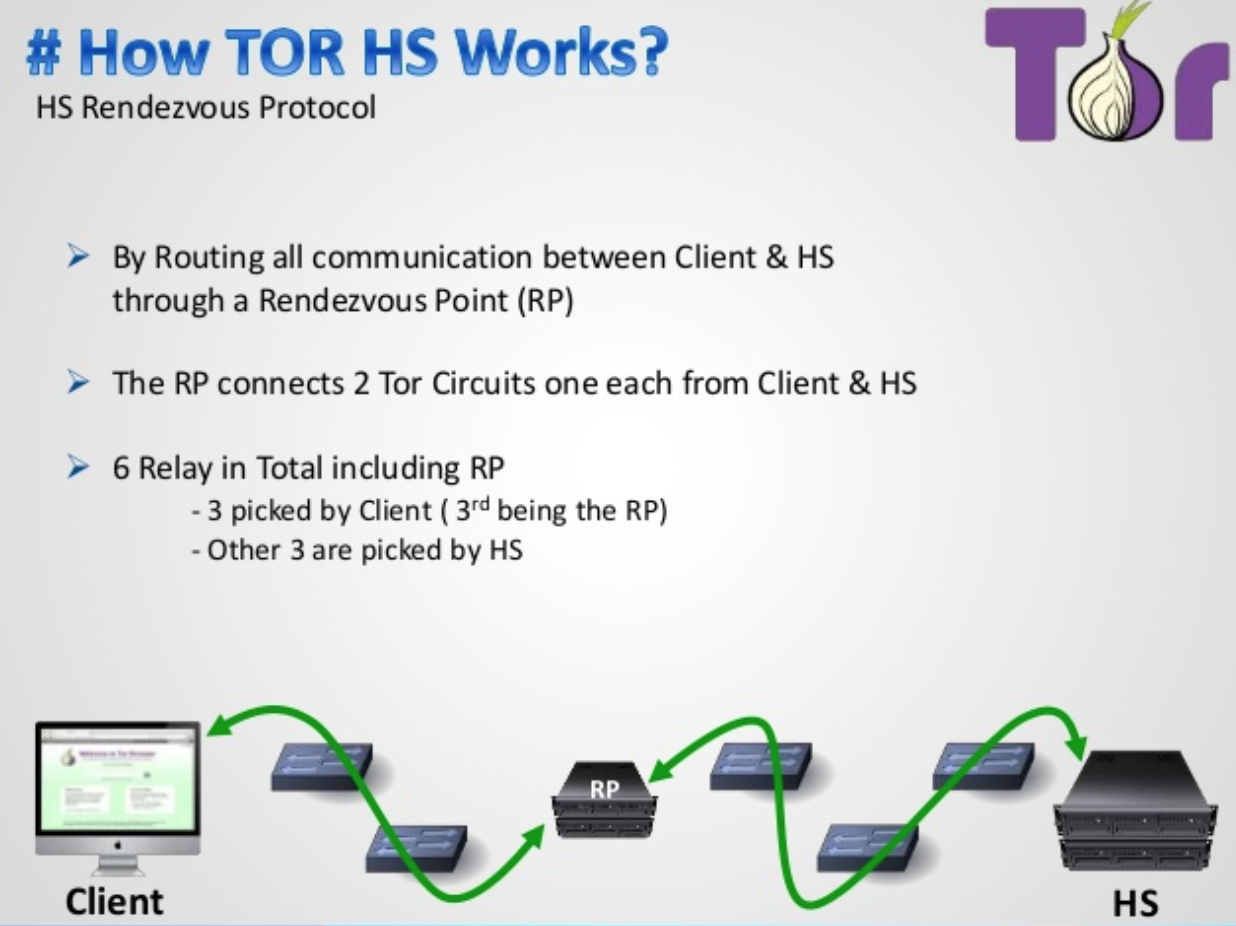
\includegraphics[scale=0.4]{HS_tor}
\caption{Tor Hidden services \cite{tor_slideshare}}
\label{fig:HS_tor} % Unique label used for referencing the figure in-text
\end{figure}

\paragraph{Up to at least October 2013 the hidden services work like this}

\begin{enumerate}
	\item A hidden service calculates its key pair (private and public key, asymmetric encryption).
	\item Then the hidden service picks some relays as its introduction points.
	\item It tells its public key to those introduction points over Tor circuits\footnote{We need to understand message formats for this action} .
	\item After that the hidden-service creates a hidden service descriptor, containing its public key and what its introduction points are.
	\item The hidden service signs the hidden service descriptor with its private key.
	\item It then uploads the hidden service descriptor to a distributed hash table (DHT).
	\item Clients learn the .onion address from a hidden service out-of-band. (e.g. public website) \footnote{A hash.onion is a 16 character name derived from the service's public key.}
	\item After retrieving the .onion address the client connects to the DHT and asks for that hash.
	\item If it exists the client learns about the hidden service's public key and its introduction points.
	\item The client picks a relay at random to build a circuit to it, to tell it a one-time secret. The picked relay acts as rendezvous point.
	\item The client creates an introduce message, containing the address of the rendezvous point and the one-time secret, before encrypting the message with the hidden service's public key.
	\item The client sends its message over a Tor circuit to one of the introduction points, demanding it to be forwarded to the hidden service.
	\item The hidden service decrypts the introduce message with its private key to learn about the rendezvous point and the one-time secret.
	\item The hidden service creates a rendezvous message, containing the one-time secret and sends it over a circuit to the rendezvous point.
	\item The rendezvous point tells the client that a connection was established.
	\item Client and hidden service talk to each other over this rendezvous point. All traffic is end-to-end encrypted and the rendezvous point just relays it back and forth. Note that each of them, client and hidden service, build a circuit to the rendezvous point; at three hops per circuit this makes six hops in total \ref{fig:HS_circuit_tor} .

\end{enumerate}

\begin{figure}[h]
\centering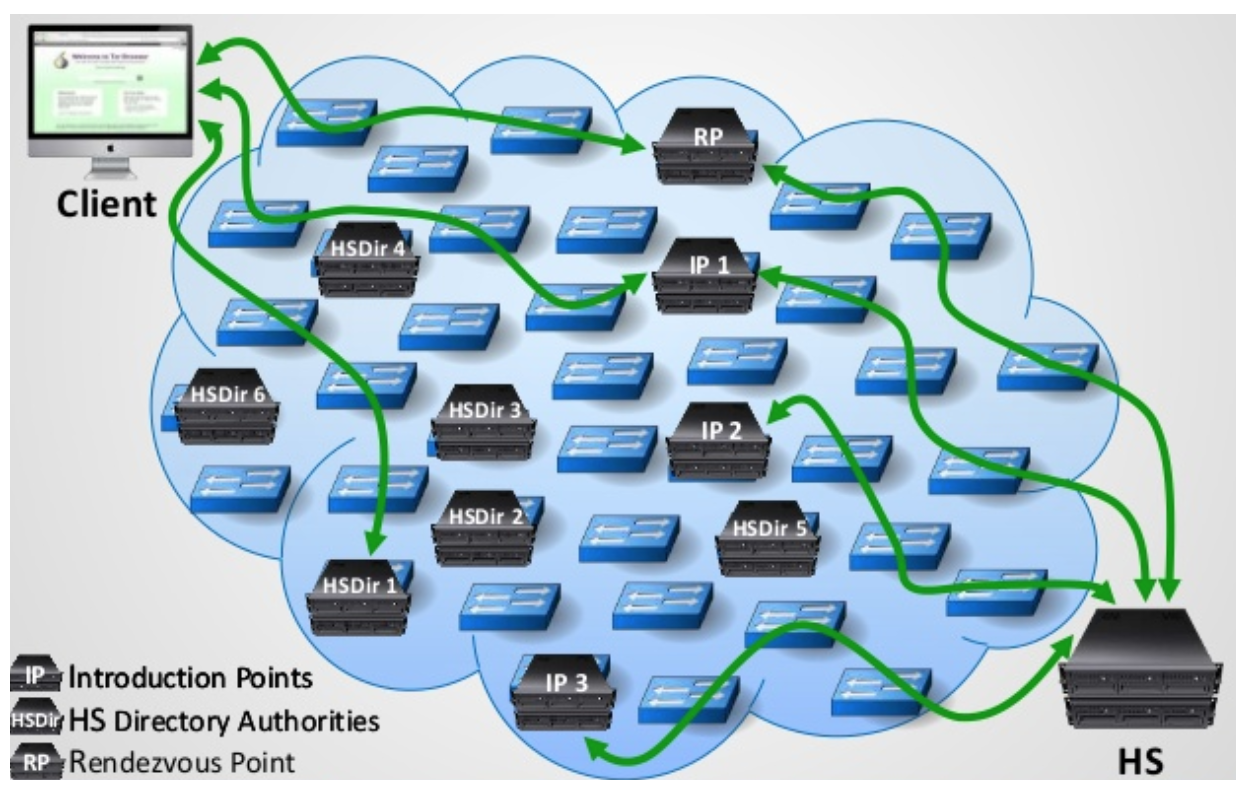
\includegraphics[scale=0.5]{HS_circuit_tor}
\caption{Tor Hidden services and HS directories \cite{tor_slideshare}}
\label{fig:HS_circuit_tor} % Unique label used for referencing the figure in-text
\end{figure}






